\section{Photon Tagger} \label{sec:clas.tagr}

The electron beam delivered to hall \desg{B} from \abbr{CEBAF} can be sent directly to a target or the electron beam can produce a \emph{real photon} beam by means of bremsstrahlung radiation by passing the electron beam through a radiator. Typical radiators have high atomic number to help reduce contamination of photons produced by electron-electron scattering. The \g12 experiment used a gold (\abbrlc{A}{u}) foil of $10^{-4}$~radiation length. This choice has a double purpose, to maximize the probability of the electron-nucleus interaction given that the bremsstrahlung cross section is proportional to $\mathrm{Z^{2}}$, and to minimize the number of interaction centers such that each electron interacts once, producing only one photon. After the electron beam passes through the radiator, the beam becomes a mixture of photons and electrons that did not interact with the radiator and recoil electrons. The mixed beam then travels into a dipole magnetic field which sweeps the electrons out of the electron-photon beam. The electrons present in the electron-photon beam are directed toward two hodoscope planes, each made of an overlapping array of scintillators to detect the energy-degraded electrons.

%  

The first scintillator plane, referred to as the E-plane (Figs.~\ref{fig:jlab.tagr.energies}, and~\ref{fig:jlab.tagr.paddles}), is used to determine the momentum of the recoiling electrons. The E-plane provides photon energy resolution on the order of 0.1\% of the incident electron beam energy. It consists of 384 paddles that are 20 cm long, 4 mm thick and from 6 to 18 mm wide. The paddles are arranged in an overlapping fashion, thus increasing the number of logical paddles to 767.
The trajectory of an electron or any charged particle in the magnetic field is governed by the equation
\begin{equation}\label{eq:motioninmag}
	p = qrB \ (\mathrm{if}\ \vec{p} \perp \vec{B} )
\end{equation}
where $p$ is the particle's momentum, $q$ is the particle's charge, $r$ is the particle's radius of curvature and $B$ is the magnetic field the particle passes through.
By determining which paddle an electron hit we know the radius of curvature and we can calculate the momentum of the electron. The momentum of the electron can then be used to obtain the energy of the photon by means of the conservation relation 
\begin{equation}\label{eq:tagger.energy}
	E_{\gamma} = E_{0} - E_{e}
\end{equation}
where $E_{0}$ is the energy of the incident electron given by \abbr{CEBAF}, $E_{e}$ is the energy of the recoil electron and $E_{\gamma}$ is the energy of the emitted photon. 

The second scintillator plane, referred to as the T-plane, is used to make accurate timing measurements of the recoiling electrons. This plane comprises of 61 paddles that are each 2 cm thick. The added thickness of these paddles allow for a timing resolution of 110 ps.
% The spectrometer was able to tag photons ranging from 20-95\% of the incident electron beam energy.

The tagger can tag photons of energies from 20 to 95\% of the incident electron beam energy. For \g12 this corresponds to a photon energy range of 1.142 - 5.425~GeV. Due to the high current of the electron beam delivered to \g12 from \abbr{CEBAF} there were usually more than one ``hit'' in the tagger for each event. Normally, the one associated with the photon that caused the event could be obtained by a timing coincidence with the tracks, although there are cases when this photon is ambiguous as discussed in Sec.~\ref{sec:analysis.beam}.

The photons that pass through the radiator then pass through a 6.2~mm diameter collimator. Collimation is used to trim the beam halo prior to arriving at the CLAS cryotarget. In the \g12 experiment the beam entering the cryotraget was 1.5~cm in radius. The collimator was positioned 537~cm upstream of the cryotarget which had a radius of 2~cm. A sweeping magnet were placed after the collimator to remove any charged particles created by interactions of photons with the collimator.

More detailed information on the Hall B tagging system and \abbr{DAQ} of the tagger system can be found in \cite{clas.tagger}.

\begin{figure}\begin{center}
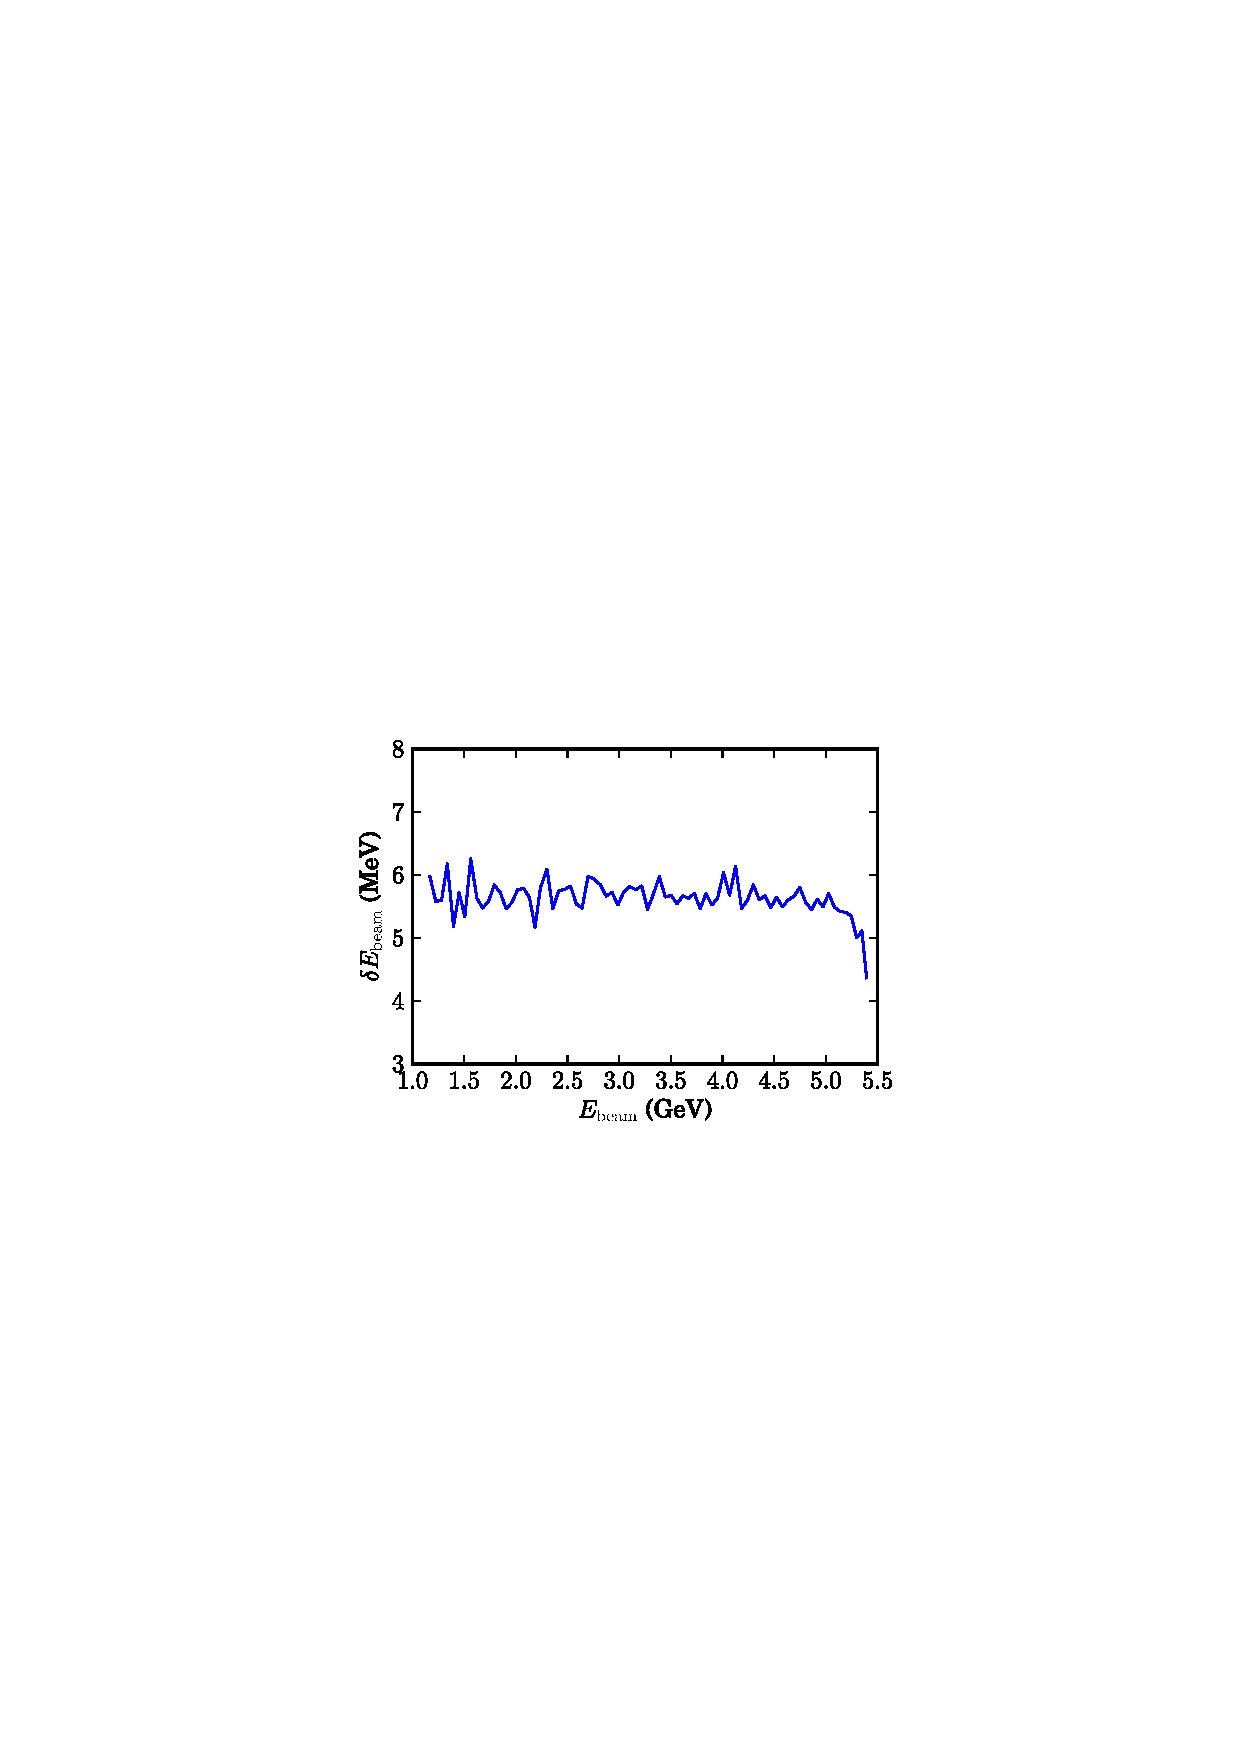
\includegraphics[width=0.8\figwidth,height=\qfigheight]{\grpath/hall-b/tagger_energies.pdf}
\caption[Scale drawing of the photon tagger system]{\label{fig:jlab.tagr.energies}Scale drawing of the photon tagger system. The rectangular area around the $E$ and $T$-counter planes outlines the expanded view shown in Fig.~\ref{fig:jlab.tagr.paddles}.}
\end{center}\end{figure}


\begin{figure}\begin{center}
\includegraphics[width=1.1\figwidth,height=\qfigheight]{\grpath/hall-b/tagger_paddles.pdf}
\caption[Scale drawing of the $E$-counters (blue) and the $T$-counters (green) showing examples of recoiled electrons (red lines) entering from the upper left]{\label{fig:jlab.tagr.paddles}{\coloronline}Scale drawing of the $E$-counters (blue) and the $T$-counters (green) showing examples of recoiled electrons (red lines) entering from the upper left.}
\end{center}\end{figure}
\FloatBarrier
